\RequirePackage{xcolor}
\documentclass[portrait,20pt]{sciposter}

% load settings
\input{settings}

\title{Title of the Poster}

% note: only give author names, not institute
\author{John Doe}
 
% insert correct institute name
\institute{Institute for Medical Engineering,\\
           Otto von Guericke University Magdeburg, Germany\\}

% shows author email address below institute
\email{john.doe@ovgu.de}

%\date is unused by the current \maketitle

% adjust the width of the logos and the title
%\setlength{\logowidth}{0.24\textwidth}
%\setlength{\titlewidth}{\textwidth}
%\addtolength{\titlewidth}{-2\logowidth}

% The following commands can be used to alter the default logo settings.
\leftlogo[1.2]{logos/logos} % defines logo to left of title (with scale factor)
%\rightlogo[1.0]{logos/emvlogo} % same but on right
\norightlogo % same as \rightlogo{}, but also widens space available for title.

% begin of Document
\begin{document}

% define conference poster is presented at (appears as footer)
\conference{Presented at the \enquote{Title of the Conference}, City, Country, Year}

\maketitle\vspace{-1em}

% begin of multicols enviroment
\begin{multicols}{3}

\section{Introduction}

\begin{block}{Why to give a poster:}
	\begin{itemize}
		\item show the main arguments and results of your work
		\item produce interest to read the full paper/report
		\item goal: be educational and also entertaining
	\end{itemize}
\end{block}

\begin{block}{Advantages of using \LaTeX ~with the \texttt{sciposter} package:}
	\begin{itemize}
		\item very easy if the report is already written in \LaTeX
		\item different themes which are usable in practice
		\item possibility to adopt presentation slides using \emph{beamerarticle}
	\end{itemize}
\end{block}

\section{Body}

\subsection{Equations}

\begin{block}{Pythagoras theorem:}
	\begin{equation}
		a^2 + b^2 = c^2 \label{eq:pythogoras}
	\end{equation}	\end{block}
	
\begin{block}{It follows that:}
	\begin{align}
		a^2 &= c^2 - b^2 \\
		b^2 &= c^2 - a^2
	\end{align} 	
\end{block}

\subsection{Tables}

\begin{table}
	\caption{Example table}
	\label{tab:example}
	\centering
		\begin{tabular}{cc}
			\toprule
			variable & meaning \\
			\midrule
			$t$ & time \\
			$U$ & voltage \\
			\bottomrule
		\end{tabular}
\end{table}

\subsection{Figures}

\begin{figure}
	\centering
		\includegraphics[width=0.7\columnwidth]{logos/unilogo}
	\caption{Logo of the university.}
	\label{fig:unilogo}
\end{figure}

\begin{figure}
	\centering
		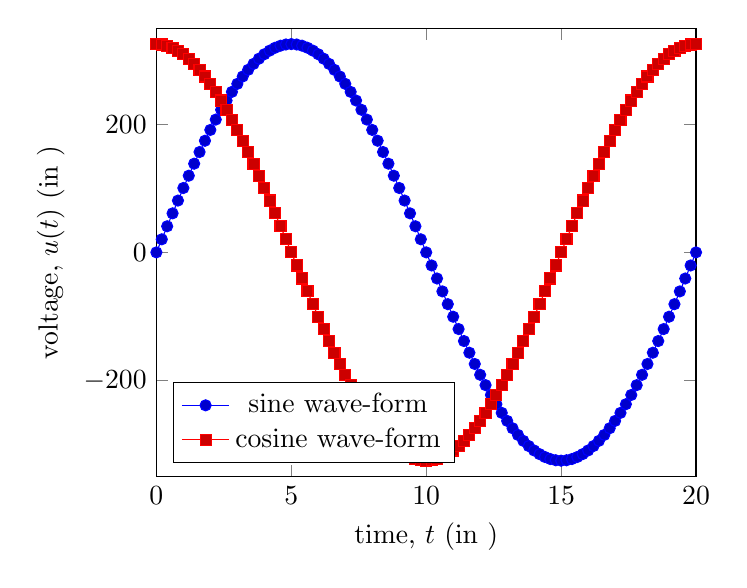
\begin{tikzpicture}
			\begin{axis}[
				xlabel={time, $t$ (in \si{\milli\second})},
				ylabel={voltage, $u(t)$ (in \si{\volt})},
				xmin=0,xmax=20,
				ymin=-350,ymax=350,
				legend pos=south west,
				% example how to insert a line by giving a formula directly
				]
				\addplot+[
					domain=0:20,
					samples=101,
				] {sin(deg(x*2*pi/20))*sqrt(2)*230};
				\addlegendentry{sine wave-form};
				\addplot+[
					domain=0:20,
					samples=101,
				] {cos(deg(x*2*pi/20))*sqrt(2)*230};
				\addlegendentry{cosine wave-form};
			\end{axis}
		\end{tikzpicture}
	\caption{Harmonic time course of a voltage with a frequency of \SI{50}{\hertz} 
	and an effective value of \SI{230}{\volt}}
	\label{fig:u_t_sinus}
\end{figure}

\begin{block}{Citations:}
	\begin{itemize}
		\item you may use short citations like~\cite{grossman:chicago_manual}
		\item people can look up the numbers in the list of references
		\item alternative: use full citations instead
	\end{itemize}
\end{block}
\begin{block}{Example for a full citation:}
	\small\fullcite{hering:technical_reports}
\end{block}

\section{Summary and Outlook}

\begin{block}{Conclusion:}
	\begin{itemize}
		\item summarize the main results of your work
		\item also talk about remaining tasks or problems	  	
	\end{itemize}
\end{block}

\begin{block}{Outlook:}
	\begin{itemize}
		\item What research questions are still open?
		\item Where would you continue if you have more time?
	\end{itemize}
\end{block}	

\begin{block}{Download from \url{http://www.insert.your.url/} or via QR Code:}
	\begin{center}
		\qrcode[height=0.7\columnwidth]{http://www.insert.your.url}
	\end{center}
\end{block}

\end{multicols}

% references section
\printbibliography

\end{document}
